\documentclass{article}      % Specifies the document class 
\usepackage{graphics, amsmath}
\usepackage{hyperref}
                             % The preamble begins here.
\title{Theory Plug-in User Manual}  % Declares the document's title.
\author{Issam Maamria \\ University of Southampton}      % Declares the author's name.
\date{\today}      

\begin{document}             % End of preamble and beginning of text.

\maketitle
The Theory plug-in is a contribution to the Rodin platform that facilitates the \textbf{specification}, \textbf{validation}, \textbf{deployment} and \textbf{use} of language and proof extensions for the Event-B methodology. Language extensions are additions to the Event-B mathematical language in the form of 1) operators and 2) datatypes. Proof extensions are additions to the Event-B proving infrastructure in the form of rewrite rules, inference rules and polymorphic theorems. The specification of extensions is achieved by means of \textit{theories} 
\includegraphics{images/thy.png}. The validation of extensions is achieved by means of proof obligations whenever appropriate. This user manual provides a comprehensive overview of the plug-in's functionality and capabilities.
\par
For a quick start guide, the user can skip to Section \ref{quickStart}.


\includegraphics[width=7mm]{images/info.png} The Event-B \textbf{mathematical language} refers to the language used to write axioms, invariants, guards etc. in Event-B models.\\


\includegraphics{images/info.png} Event-B theories are Rodin file just like contexts and machines.

\section{Motivation}
Work on the Theory plug-in started as an effort to create a \textit{Rule-based Prover} for Event-B much like the ML prover in Atelier-B. The Rule-based Prover, as it was known then, supported the definition, validation and use of rewrite rules. The Theory plug-in is the successor of the Rule-based Prover, and offers much more functionality.
\par 
Prior to Rodin v2.0, the mathematical language used in Event-B was fixed. As such, it was not possible to define reusable polymorphic operators. A workaround was to define any required operators as set constructs in contexts. Originally, contexts were supposed to provide a parametrization of machines. The aforementioned limitations of the Event-B language lead to users to use contexts for purposes for which they were not intentionally devised. Examples of operators that can be useful to users include the sequence operator (which was present in classical B mathematical language) and the bag operator.
\par
In Rodin v2.0, a dynamic parser has been implemented for the Event-B AST. The Theory plug-in was a natural candidate for defining and using mathematical extensions. To provide a comprehensive platform, cover for a wider range of proof rules was also needed.


\includegraphics{images/info.png} ML is a rule-based prover as opposed to the semi-decision procedure PP.

\section{Capabilities}
The Theory plug-in has the following capabilities:
\begin{enumerate}
	\item \textbf{\textit{Theory Definition:}}
		\begin{enumerate}
			\item Definition of \textbf{datatypes}: datatypes are defined by supplying the types on which they are polymorphic, a set of constructors one of which has to be a base constructor. Each constructor may or may not have destructors.
			\item Definition of \textbf{operators}: operators can be defined as predicate or expression operators. An expression operator is an operator that "returns" an expression, an example existing operator is $card$. A predicate operator is one that "returns" a predicate, an example existing predicate operator is $finite$.
			\item Definition of \textbf{rewrite rules}: rewrite rules are one-directional equalities that can be applied from left to right. The Theory plug-in can be used to define rewrite rules.
			\item Definition of \textbf{inference rules}: inference rules can be used to infer new hypotheses, split a goal into sub-goals or discharge sequents.
			\item Definition of \textbf{polymorphic theorems}: theorems can be defined and validated once, and can then be imported into sequents of proof obligations if a suitable type instantiation is available.
			\item \textbf{Validation of extensions}: where appropriate, proof obligations are generated to ensure soundness of extensions. This includes, proof obligations for validity of inference and rewrite rules, as well as proof obligations to validate operator properties such as associativity and commutativity.
		\end{enumerate}
	\item \textbf{\textit{Theory Deployment:}} this step signifies that a theory is ready for use. Theories can be deployed after they have been optionally validated by the user. It is strongly advisable to discharge all proof obligations before deployment.
\end{enumerate}
Once a theory has been deployed to its designated project, all its extensions (mathematical and proof extensions) can be used in models. In later sections, we show the two different scopes of theory availability.
\\
\\

\includegraphics{images/info.png} In the Event-B mathematical language, predicates (known as formulae in most literature) and expressions (known as terms) are two separate syntactic categories. Expressions have a type. Predicate do not.
\section{Quick Start}\label{quickStart}
In this section, we step through a simple tutorial on how to define and use a simple theory.
Click on the links above to navigate through this tutorial.
\subsection{Install Theory Plug-in}
The installation or update for the Theory plug-in is available under the main Rodin Update site (\url{http://rodin-b-sharp.sourceforge.net/updates}) under the category "Modelling Extensions". Like always, after the installation, restarting Rodin is recommended. For more details, see \url{http://wiki.event-b.org/index.php/Theory_News_and_Support}.

\begin{center}
\begin{figure}
\label{newTFW}
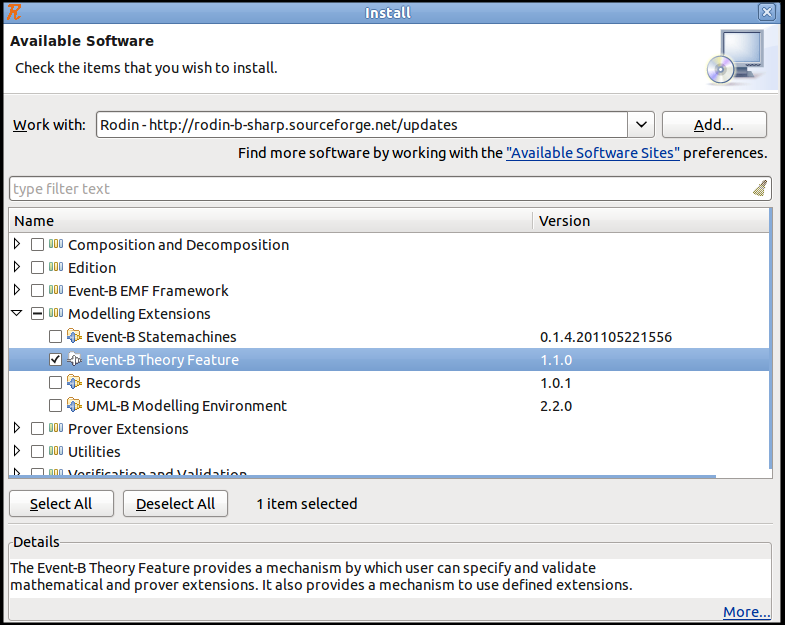
\includegraphics{images/InstallTheory.png}
\caption{Install Theory Plug-in}
\end{figure}
\end{center}

Once the Theory plug-in is successfully installed, menu entries will be added in certain places. In particular, the Event-B Explorer will have an additional button 
\includegraphics{images/newThy.png} that initiates the wizard to create new theory files.

\begin{center}
\begin{figure}
\label{newTFW}
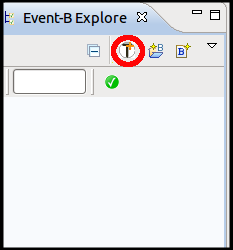
\includegraphics{images/NewTheoryButton.png}
\caption{New Theory Button in Event-B Explorer}
\end{figure}
\end{center}

\subsection{Create A New Theory}
An additional button 
\includegraphics{images/newThy.png} (red-circled below) should appear in the Event-B Explorer.

\begin{center}
\begin{figure}
\label{newTFW}
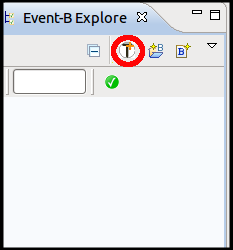
\includegraphics{images/NewTheoryButton.png}
\caption{New Theory Button in Event-B Explorer}
\end{figure}
\end{center}

\par 
By clicking the button 
\includegraphics{images/newThy.png}, a wizard that enables the creation of a new theory is initiated. Figure 4 shows the wizard in action.

\begin{center}
\begin{figure}
\label{newTFW}
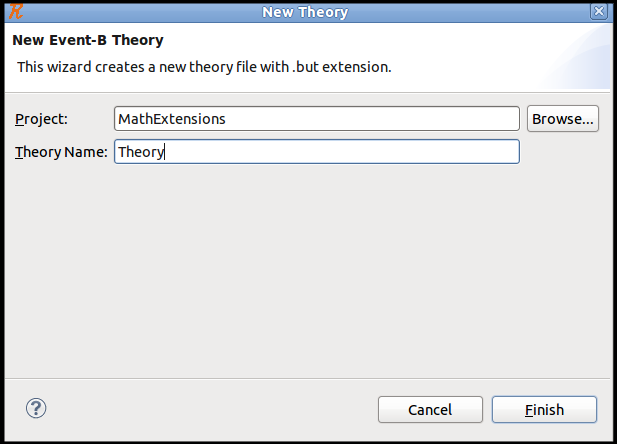
\includegraphics{images/NewTheoryWizard.png}
\caption{New Theory File Wizard}
\end{figure}
\end{center}


\includegraphics{images/info.png} Note that, as a side effect of pressing the 
\includegraphics{images/newThy.png} button, a project called \textbf{"MathExtensions"} is created. This is the project in which \textit{global} theories reside.
\par 

\par
In the wizard, specify the parent project of the theory and a theory name. The project can be selected using the button on the right hand side of project name text field (akin to selecting a project when creating a new Event-B component). Click the Finish button to create the theory.
\par 
If there are no name clashes between the name of the new theory and any existing resources, you should get a theory editor opened up as depicted in Figure 5.
\begin{center}
\begin{figure}
\label{theoryEditor}
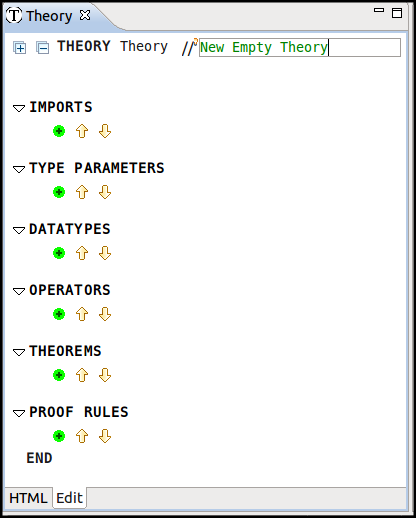
\includegraphics{images/TheoryEditor.png}
\caption{The Theory Editor}
\end{figure}
\end{center}

\par 
The theory editor has two pages: an Edit page and an HTML (i.e., pretty print) page. The edit page corresponds to the structured editor. The HTML page is a pretty print view of the theory.

\subsection{Add a Type Parameter}
Type parameters in a theory specify the types on which new definitions and rules may be polymorphic. For instance, a theory of sequences can be polymorphic on one type and that is the type of elements it may hold.
\par 
Type parameters are similar in nature to carrier sets in contexts. To create a new type parameter, click on button 
\includegraphics{images/add.png} under the Type Parameters section of the structured editor, and specify the name of the type parameter (see Figure 6).

\begin{center}
\begin{figure}
\label{typePar}
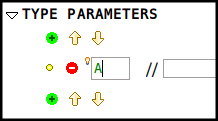
\includegraphics{images/TypeParameter.png}
\caption{Type Parameters}
\end{figure}
\end{center}


\includegraphics{images/note.png} Type parameters are expected to be a legal Event-B identifier. For example, $2ident$ is not a legal identifier.


\includegraphics{images/nike.png} As a convention, type parameters are specified as upper case strings (same as context's carrier sets).

\subsection{Create an Operator Definition}
Event-B mathematical language has many useful operators. Examples include cardinality operator $card$, the finiteness predicate operator $finite$ and the function application $.(.)$. Other useful operators can be defined using the Theory plug-in. The following figure shows a definition of a sequence operator.

\begin{center}
\begin{figure}
\label{seqOP}
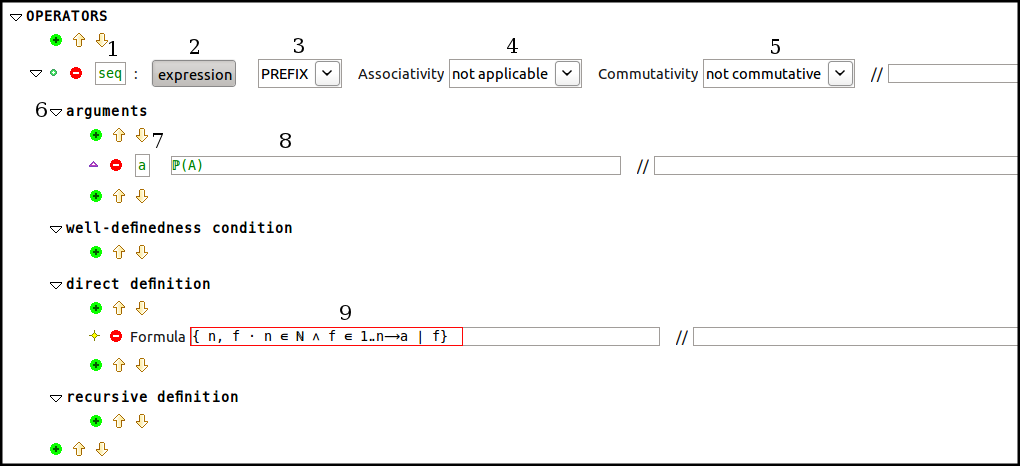
\includegraphics{images/SeqOperator.png}
\caption{Sequence Operator Definition}
\end{figure}
\end{center}

Note the numbering in the above picture. The following explains each part of the definition:
\begin{enumerate}
	\item \textbf{Syntax Symbol}: this specifies the syntax token that will be reserved for the new operator (sequence in our example). It should not clash with any previously defined symbol in the mathematical language available to the theory.
	\item \textbf{Syntactic Class}: this specifies whether the new operator is an expression operator or a predicate operator. For example, the cardinality operator $card$ is an expression operator of integer type, and the finiteness operator $finite$ is a predicate operator. In our case, the sequence operator is an expression operator. The button can be toggled off if a predicate operator is required instead.
	\item \textbf{Notation}: this specifies whether the symbols is a prefix or an infix operator. In the existing mathematical language, $+$ is an infix operator whereas $partition$ is a prefix predicate operator. In our example, the sequence operator is specified as prefix.
	\item \textbf{Associativity}: this specifies whether the operator is associative. Note that this has semantic implications, and as such a proof obligation is generated to check the associativity property.
	\item \textbf{Commutativity}: this specifies whether the operator is commutative. Note that this has semantic implications, and as such a proof obligation is generated to check the commutativity property.
	\item \textbf{Operator Arguments}: an operator may have a number of arguments (all of which may be expressions).
	\item \textbf{Argument Identifier}: this specifies the name of the argument of the operator. It has to be a legal Event-B identifier (similar to carrier sets, constant, variables etc.).
	\item \textbf{Argument Type}: this specifies the type of the argument. In our case, the sequence operator takes a set of type $A$. Since $A$ is a type parameter, the sequence is polymorphic.
	\item \textbf{Direct Definition}: this provides the direct definition of the operator. In our case (see the red-boxed field), it asserts that sequences are total functions from a contiguous integer range starting at 1 to the set $a$ the argument of the operator $seq$. 
\end{enumerate}


\includegraphics{images/info.png} 
\begin{itemize}
	\item Only operators that take two arguments of the same type can be tagged as commutative. Of course, then, one has to prove the mathematical property.
	\item An operator can be tagged as being associative if it satisfies the three conditions: (1) it is an expression operator, (2) it takes two (or more) arguments of the same type, (3) the type of the operator is the same as that of its arguments. Of course, then, one has to prove the mathematical property.
	\item Operators that are tagged associative have to be tagged as infix as well.
	\item The argument type can be a type or a set expression. If the argument type is a set expression, then the type of the argument is inferred. Furthermore, the additional restriction (i.e., that the argument belongs to a set expression) is added as a well-definedness condition for the operator.
\end{itemize}


\includegraphics{images/nike.png} 
\begin{itemize}
	\item As a convention, names of operators should be lower case.
	\item As a convention, names of operator arguments should be lower case.
\end{itemize}

\par 
The following operator defines size for sequences.

\begin{center}
\begin{figure}
\label{seqOP}
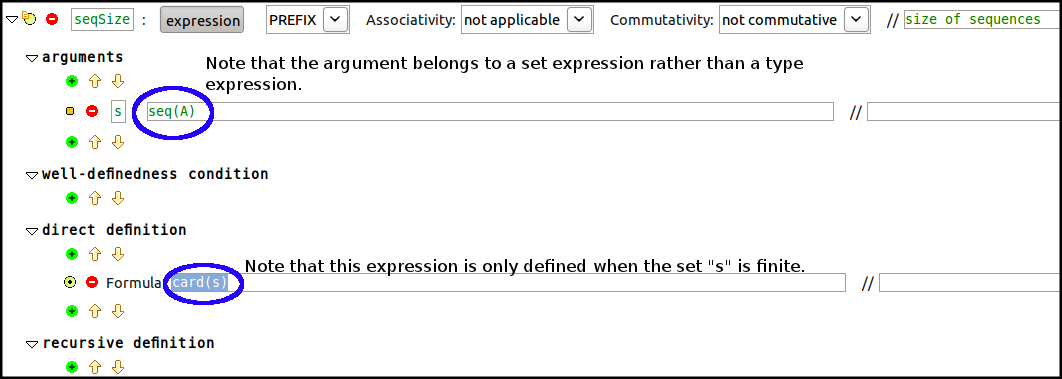
\includegraphics{images/SeqSize.png}
\caption{Sequence Size Operator Definition}
\end{figure}
\end{center}

This definition asserts that the operator $seqSize$ takes one argument of type $\mathbb{Z} \leftrightarrow A$.
This definition, also, triggers a proof obligation to prove the strength of the well-definedness condition provided. Namely, one has to prove that $\forall s \cdot s \in seq(A) \Longrightarrow finite(s)$. We leave this as an exercise to the reader.

\par 
The following is a definition of a predicate operator:

\begin{center}
\begin{figure}
\label{seqOP}
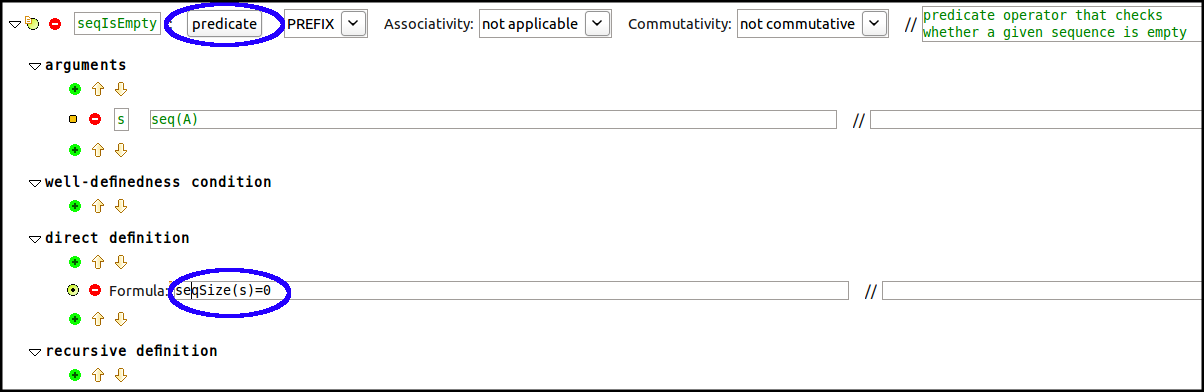
\includegraphics{images/SeqIsEmpty.png}
\caption{Sequence Size Operator Definition}
\end{figure}
\end{center}

The definition of $seqIsEmpty$ does not trigger any proof obligation for well-definedness strength. This is due to the fact that the corresponding condition is a trivial predicate, namely:
$\forall s \cdot s \in seq(A) \Longrightarrow s \in seq(A)$.

\par 
The head operator on sequences can be defined as follows:

\begin{center}
\begin{figure}
\label{seqOP}
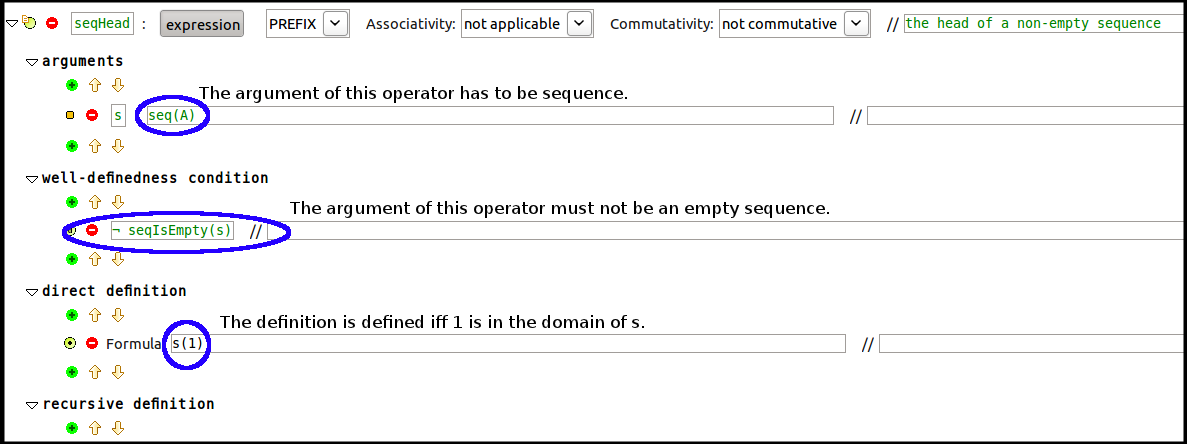
\includegraphics{images/SeqHead.png}
\caption{Sequence Head Operator Definition}
\end{figure}
\end{center}

The following figure shows the well-definedness strength proof obligation corresponding to the previous definition of $seqHead$.

\begin{center}
\begin{figure}
\label{seqOP}
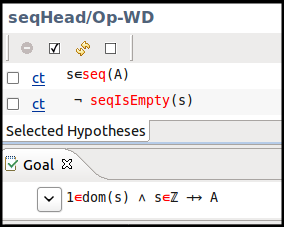
\includegraphics{images/SeqHeadPO.png}
\caption{Sequence Head WD Strength PO}
\end{figure}
\end{center}

\par 
As a summary, have a look at the following caption which is taken from the HTML view of our theory:

\begin{center}
\begin{figure}
\label{seqOP}
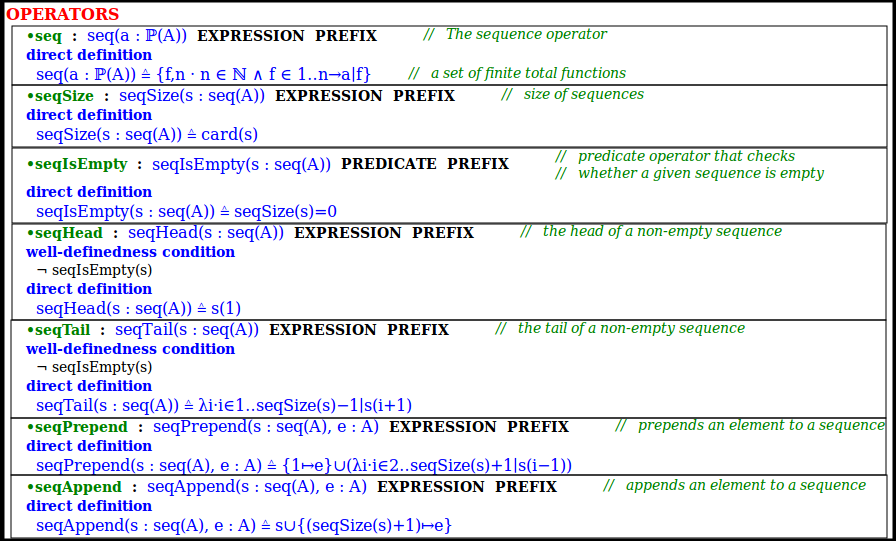
\includegraphics{images/SeqOperators.png}
\caption{Various Sequence Operators}
\end{figure}
\end{center}

The proof obligations associated with an operator definition are the following:
\begin{enumerate}
	\item \textbf{./Op-WD} operator well-definedness strength if a well-definedness condition is explicitly specified.
	\item \textbf{./Op-COMMUT} the commutativity proof obligation, generated if the operator is tagged as commutative.
	\item \textbf{./Op-ASSOC} the associativity proof obligation, generated if the operator is tagged as associative.
\end{enumerate}

\subsection{Specify a Polymorphic Theorem}
A polymorphic theorem is no different, in principle, from theorems defined in contexts and machines. The Theory plug-in, however, provides facilities to instantiate and use these theorems in proofs. See the example below.

\begin{center}
\begin{figure}
\label{theoremEx}
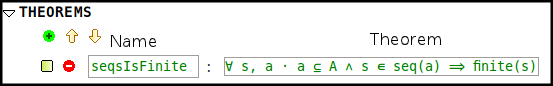
\includegraphics{images/Theorem.png}
\caption{Sequence Finiteness Theorem}
\end{figure}
\end{center}

\par 
The previous theorem articulates the fact the sequences as specified in our example are finite. As with theorems in contexts and machines, you have to prove validity and well-definedness of the theorem. The proof obligations associated with a theorem are the following:

\begin{enumerate}
	\item \textbf{./S-THM} the validity proof obligation.
	\item \textbf{./WD-THM} the well-definedness proof obligation.
\end{enumerate}

The following figure shows other theorems that can be defined in relation to our theory of sequences so far:

\begin{center}
\begin{figure}
\label{theoremsEx}
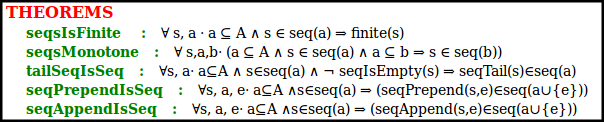
\includegraphics{images/Theorems.png}
\caption{Sequence Theorems}
\end{figure}
\end{center}


\includegraphics{images/nike.png} A theorem can be instantiated (e.g., in the previous example, the type parameter $A$ can be substituted with a type expression that is acceptable in the context of the sequent under consideration). We will later show how this is achieved.

\subsection{Specify an Inference Rule}
Inference rules are proof rules that can be used to: (1) infer new hypotheses in a proof, or (2) split the goal into sub-goals, or (3) discharge a proof obligation. The general structure of an inference rule is as follows:

\begin{eqnarray*}
	&Given& \\
	&~~~~~&G0,~...,~Gn \\
	&Infer& \\
	&~~~~~&I
\end{eqnarray*}

where each of $G0, ..., Gn$ and $I$ is an Event-B predicate. The above inference rule can be read in the following two ways : "given conditions~$G0$, ..., $Gn$~ one can infer $I$", and "one can prove $I$, if one can prove each of $G0$, ..., $Gn$".

\par 
Inference rules can be defined as part of a block of "Proof Rules". Each proof rules block may contain a number of metavariables, rewrite rules and inference rules. To create a rules block, under the heading "PROOF RULES" in the structured editor, press 
\includegraphics{images/add.png}.

\begin{center}
\begin{figure}
\label{blockEx}
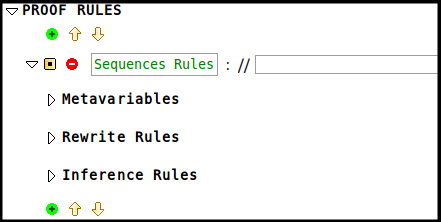
\includegraphics{images/Block.png}
\caption{Proof Rules Block}
\end{figure}
\end{center}

Metavariables define the variables used to specify proof rules. Each metavariable has a name and a type. For our example, we need one metavariable $s$.

\begin{center}
\begin{figure}
\label{metavarEx}
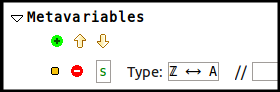
\includegraphics{images/Metavar.png}
\caption{Defining a Metavariable}
\end{figure}
\end{center}

\par 
The following example shows an inference rule concerning finiteness of sequences:

\begin{center}
\begin{figure}
\label{infEx}
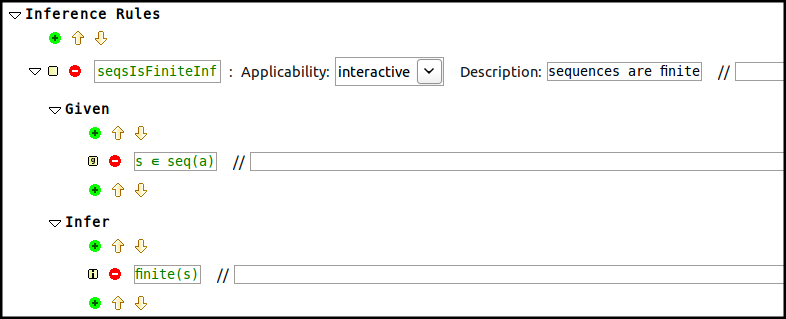
\includegraphics{images/Inference.png}
\caption{Sequence Finiteness Inference Rule}
\end{figure}
\end{center}

\par 
The applicability of a proof rule indicates whether the rule should be applied automatically or interactively. The description provides a human-readable view of the rule. The description provided will be the tool tip for the rule in the proof UI. The following inference rule is an automatic rule that states that the tail of a non-empty sequence is a sequence.

\begin{center}
\begin{figure}
\label{infTEx}
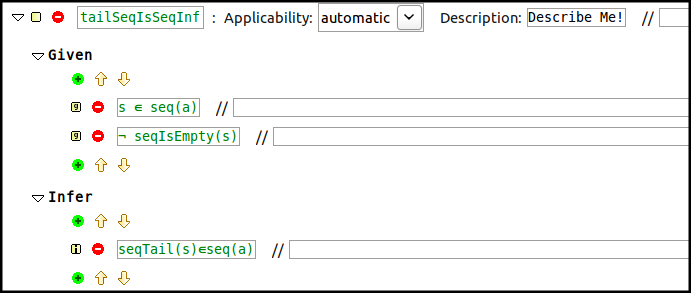
\includegraphics{images/TailInference.png}
\caption{Sequence Tail Inference Rule}
\end{figure}
\end{center}
\section{Scoping of Theories}
The MathExtensions project is created automatically if it does not exist already. The MathExtensions project is the project that should be used to develop theories that can be used by all projects. Other theories that may not be useful to all projects, but to a specific one, should be created within that project. Those theories are said to be project-scoped.
\begin{enumerate}
	\item \textbf{Workspace Scope}: Refers to the theories that reside in MathExtensions project. Deployed theories in this project are available to the entire workspace.
	\item  \textbf{Project Scope}: Theories that are not in MathExtensions are project-scoped, and are only available within the parent project.
\end{enumerate}


\section{Examples}
\subsection{Sequence}

\subsection{List}
\end{document}               % End of document.